% Mothbox Pro, notice de paramétrage sur le terrain (A4 paysage)
% Compilation : pdflatex notice-mothbox.tex (deux passes)
\documentclass[10pt,a4paper]{article}
\usepackage[T1]{fontenc}
\usepackage[utf8]{inputenc}
\usepackage[french]{babel}
\usepackage[default,semibold]{sourcesanspro}
\usepackage[landscape,top=1.5cm,bottom=1.4cm,left=1.6cm,right=1.6cm,headheight=13pt,headsep=12pt,footskip=20pt]{geometry}
\usepackage{xcolor,graphicx,tabularx,booktabs,array,enumitem,multicol}
\usepackage{fancyhdr,titlesec,tikz,fontawesome5}
\usepackage[hidelinks]{hyperref}
\usetikzlibrary{calc}

\definecolor{marque}{HTML}{2E6B4F}
\definecolor{trait}{HTML}{9A9A9A}
\definecolor{fondgris}{HTML}{F2F2F2}

\graphicspath{{annotees_notice/}{photos/}}
\setlength{\parindent}{0pt}
\setlength{\parskip}{4pt}
\setlist{itemsep=2pt,topsep=2pt,leftmargin=1.4em}
\setlist[itemize]{label=\textbullet}
\renewcommand{\arraystretch}{1.25}
\newcolumntype{L}{>{\raggedright\arraybackslash}X}

\pagestyle{fancy}
\fancyhf{}
\fancyhead[L]{\footnotesize Mothbox Pro \textbar{} Notice de paramétrage sur le terrain}
\fancyhead[R]{\footnotesize Réf. MB-NP-01 \textbar{} Rév. A}
\fancyfoot[L]{\footnotesize FR}
\fancyfoot[R]{\footnotesize \thepage}
\renewcommand{\headrulewidth}{0.4pt}

\titleformat{\section}{\Large\bfseries}{\textcolor{marque}{\thesection}}{0.6em}{}[\vspace{-6pt}\rule{\linewidth}{0.4pt}]
\titleformat{\subsection}{\normalsize\bfseries}{\thesubsection}{0.6em}{}
\titlespacing*{\section}{0pt}{2pt}{8pt}
\titlespacing*{\subsection}{0pt}{8pt}{2pt}

\newcommand{\sw}[1]{\textbf{#1}}
\newcommand{\rep}[1]{\tikz[baseline=(n.base)]\node[circle,draw,line width=0.6pt,inner sep=0.8pt,minimum size=1.15em,font=\footnotesize\bfseries](n){#1};}

\newcommand{\avert}[2]{%
  \par\smallskip\noindent
  \begin{tabularx}{\linewidth}{@{}p{0.75cm}!{\color{black}\vrule width 1.2pt}@{\hspace{6pt}}X@{}}
  \raisebox{-2pt}{\Large\faExclamationTriangle} & \textbf{#1}\quad #2
  \end{tabularx}\par\smallskip}
\newcommand{\remarque}[1]{%
  \par\smallskip\noindent
  \begin{tabularx}{\linewidth}{@{}p{0.75cm}!{\color{trait}\vrule width 1.2pt}@{\hspace{6pt}}X@{}}
  \raisebox{-2pt}{\Large\faInfoCircle} & \textbf{Remarque}\quad #1
  \end{tabularx}\par\smallskip}

% Schéma d'un bloc de switches. #1 : largeur en nombre de switches ; #2 : liste nom/état (1 = ON)
\newcommand{\dip}[2]{%
\begin{tikzpicture}[x=1.0cm,y=0.34cm,baseline=(current bounding box.center)]
  \fill[black,rounded corners=1.5pt] (0,0) rectangle (#1,2.3);
  \foreach \nom/\etat [count=\i] in {#2} {
    \fill[gray!55] (\i-0.82,0.32) rectangle (\i-0.18,1.98);
    \ifnum\etat=1
      \fill[white] (\i-0.78,0.36) rectangle (\i-0.22,1.08);
    \else
      \fill[white] (\i-0.78,1.22) rectangle (\i-0.22,1.94);
    \fi
    \node[font=\scriptsize\bfseries,anchor=south] at (\i-0.5,2.4) {\nom};
  }
  \node[font=\tiny,anchor=east] at (-0.08,0.72) {ON};
  \node[font=\tiny,anchor=east] at (-0.08,1.58) {OFF};
\end{tikzpicture}}

\begin{document}

% ---------------------------------------------------------------- Couverture
\thispagestyle{empty}
\begin{minipage}[t][17.4cm][t]{0.46\textwidth}
\vspace{0pt}
{\small\begin{tabular}{@{}l!{\color{trait}\vrule}l@{}}\textbf{PSL3D}\hspace{6pt} & \hspace{6pt}\textbf{DINALab} \\ & \hspace{6pt}Digital Naturalism Laboratories \\ \end{tabular}}\par\vspace{1.8cm}
{\fontsize{40}{44}\selectfont\bfseries Mothbox Pro}\par\vspace{6pt}
{\LARGE Notice de paramétrage\\[2pt]sur le terrain}\par\vspace{14pt}
{\color{marque}\rule{3cm}{3pt}}\par\vspace{14pt}
{\large Réglage de l'heure, du planning et test\\ de la Mothbox depuis un téléphone}\par
\vfill
\avert{Important}{Lire cette notice avant la première mise en service.}
\vspace{10pt}
{\footnotesize
\begin{tabular}{@{}ll@{}}
Logiciel & 5.2.1-webui \\
Carte électronique & Mothbox v5.0.5 \\
Référence & MB-NP-01, révision A \\
Date & novembre 2026 \\
\end{tabular}}
\end{minipage}\hfill
\begin{minipage}[t][17.4cm][c]{0.48\textwidth}
\centering
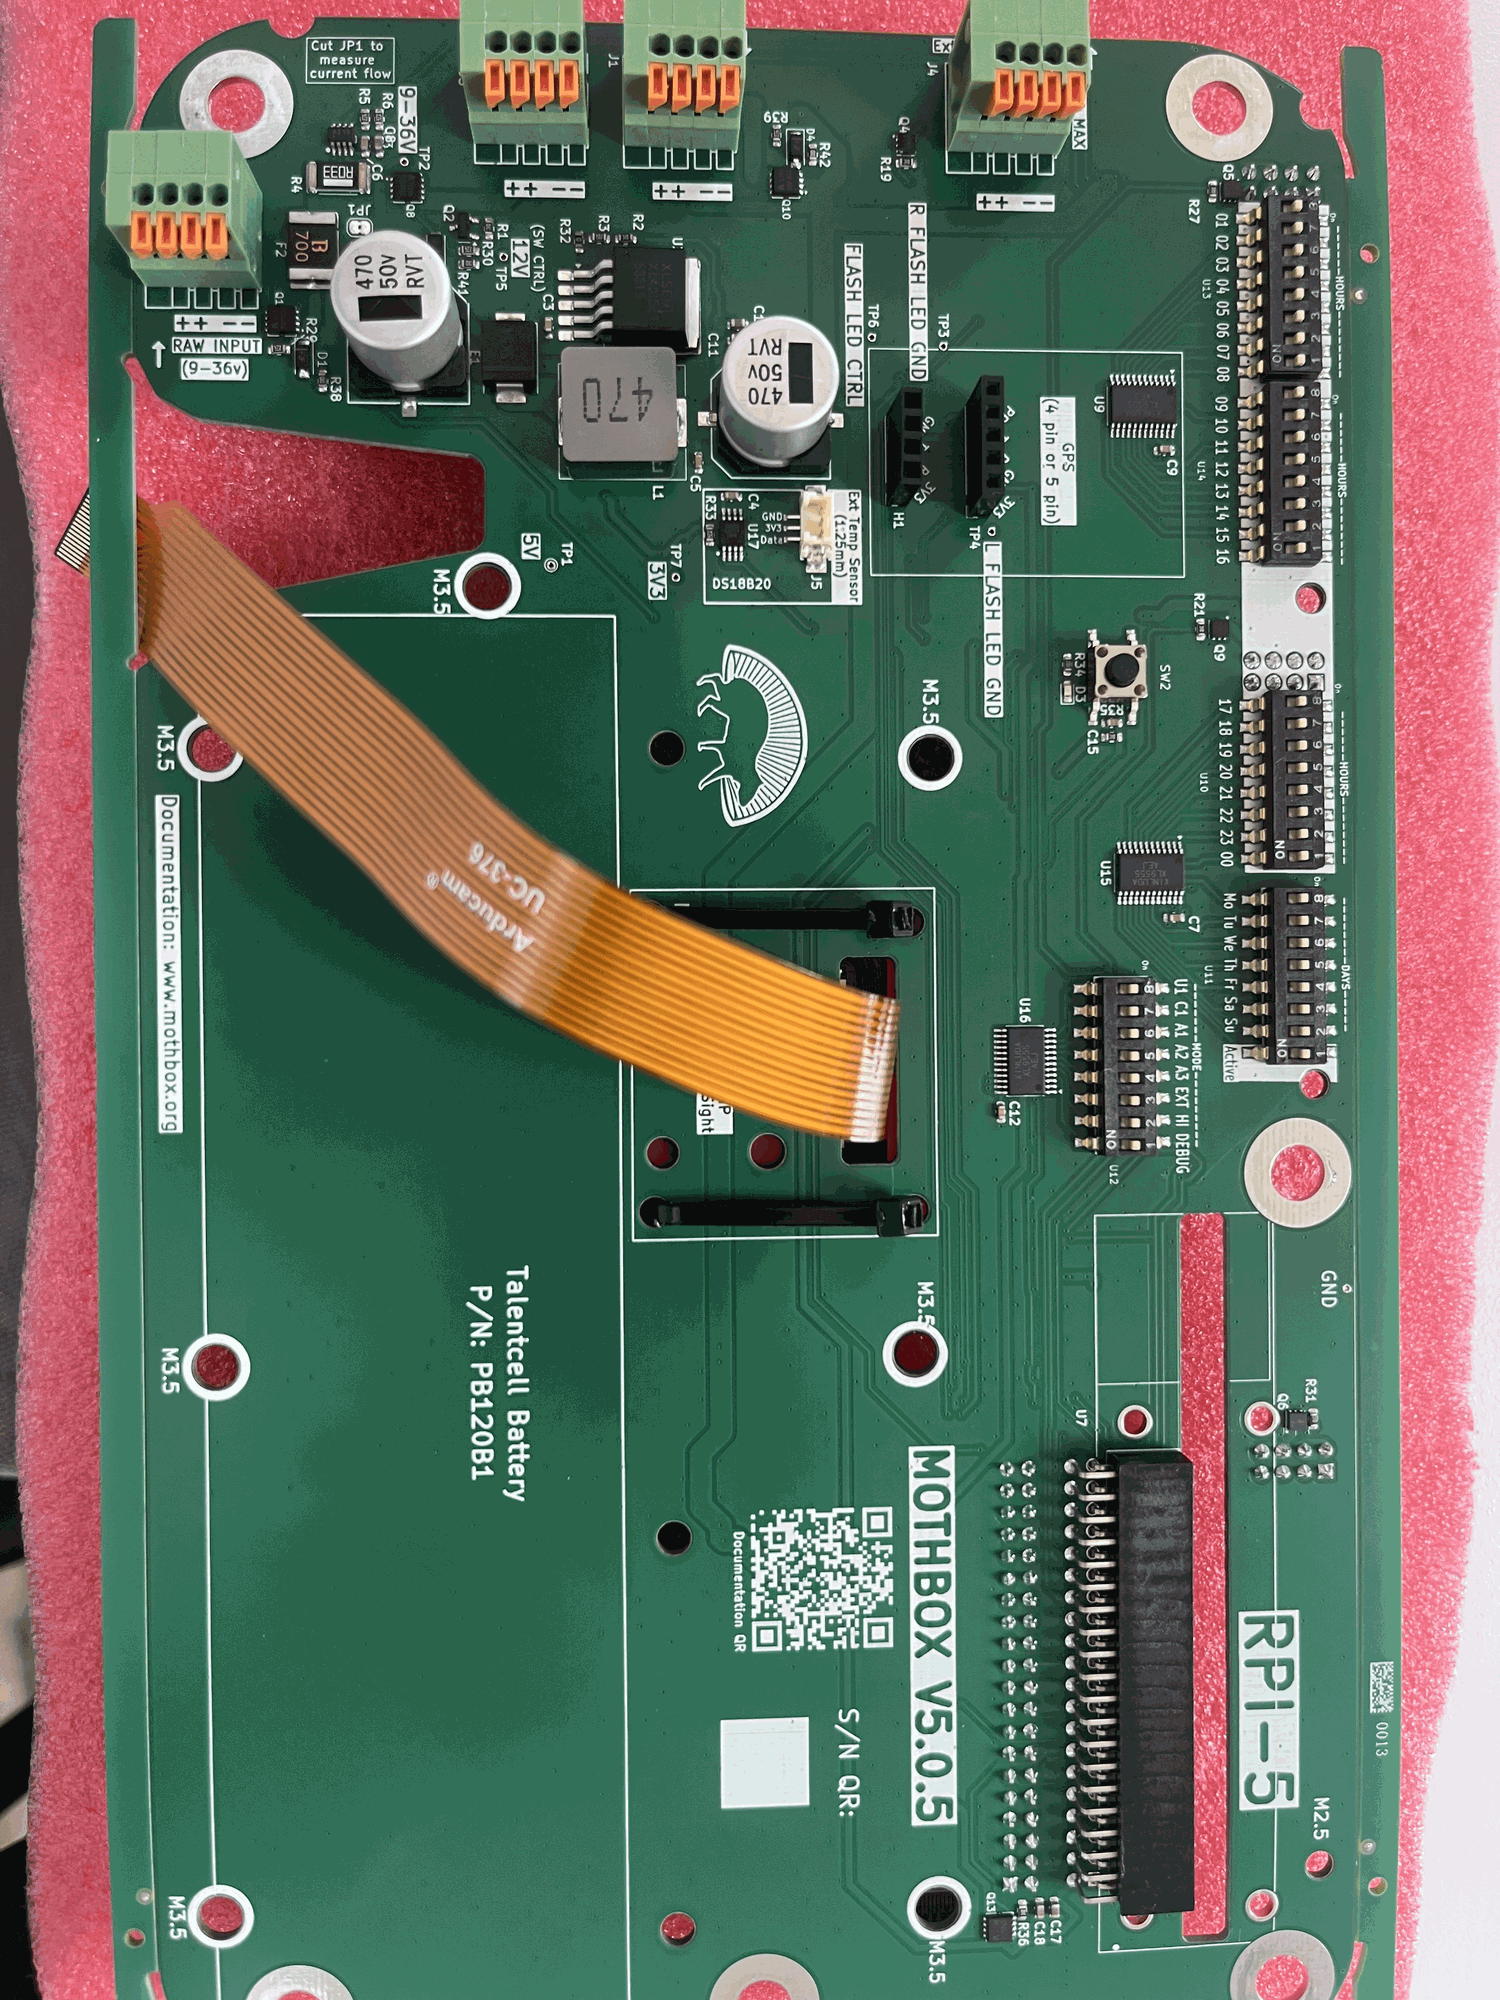
\includegraphics[height=16.8cm,trim=880 120 0 120,clip]{carte_entiere.png}
\end{minipage}

% ---------------------------------------------------------------- Page 2
\newpage
\begin{minipage}[t]{0.40\textwidth}
\vspace{0pt}
\section{Présentation}
La Mothbox se règle depuis un téléphone ou un ordinateur, sans application à installer ni connexion à Internet.

Lorsque le switch \sw{DEBUG} est sur ON, la Mothbox crée son propre réseau wifi et propose une page de réglage. Une fois les réglages terminés, \sw{DEBUG} est remis sur OFF et la Mothbox fonctionne seule selon le planning choisi.

\subsection{Éléments de la carte}
\begin{tabular}{@{}cl@{}}
\rep{1} & Switches des heures (01 à 00) \\
\rep{2} & Switches des jours (Mo à Su) \\
\rep{3} & Switch \sw{Active} \\
\rep{4} & Switch \sw{U1}, mode manuel \\
\rep{5} & Rangée MODE \\
\rep{6} & Switch \sw{DEBUG}, mode réglage \\
\end{tabular}

\section{Avant de commencer}
Matériel nécessaire :
\begin{itemize}
  \item une Mothbox équipée d'une carte SD avec le logiciel 5.2.1-webui ;
  \item une batterie chargée ;
  \item un téléphone ou un ordinateur avec wifi et navigateur web.
\end{itemize}
\avert{Attention}{Les switches ne sont lus qu'au démarrage. Après chaque changement de position, redémarrer la Mothbox.}
\end{minipage}\hfill
\begin{minipage}[t]{0.55\textwidth}
\vspace{0pt}\centering
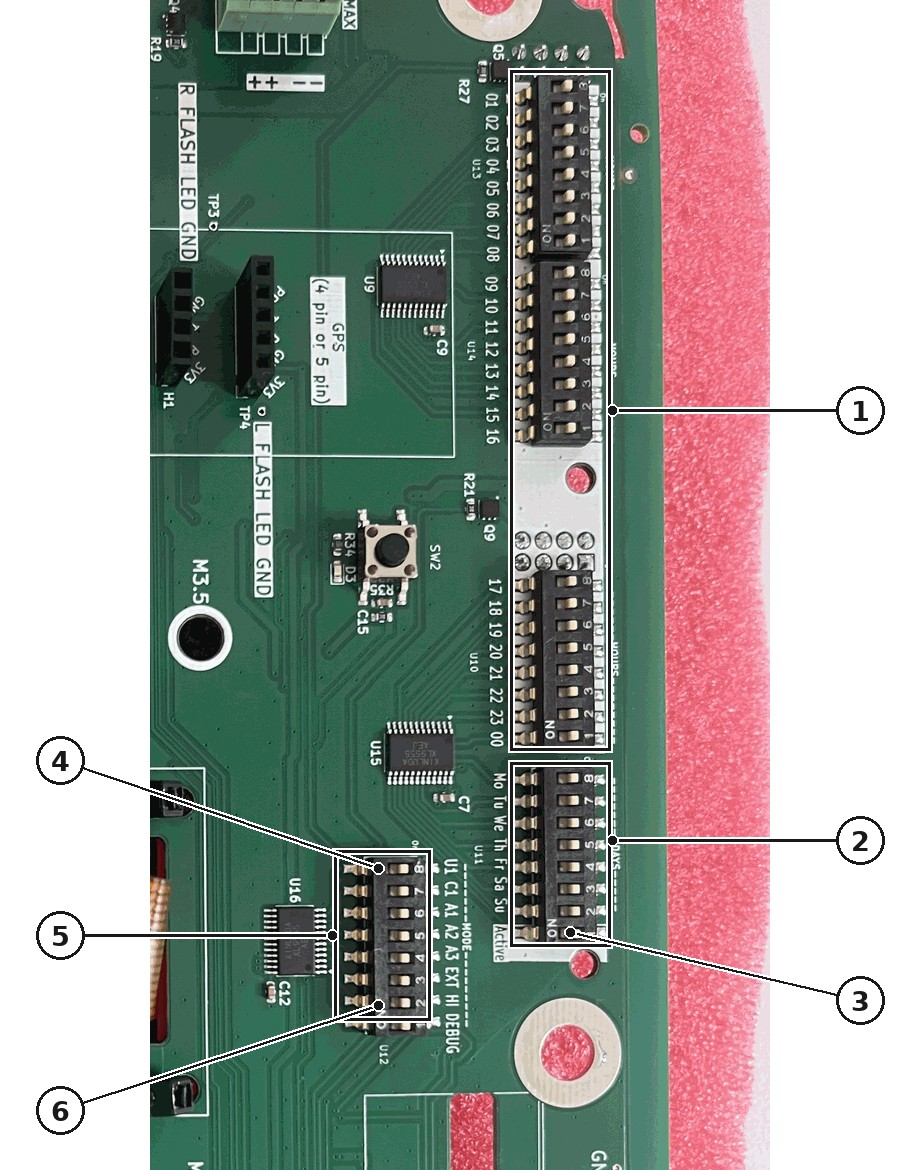
\includegraphics[height=16.6cm]{carte.jpg}\par
{\footnotesize Figure 1 : carte Mothbox v5.0.5, zone des switches}
\end{minipage}

% ---------------------------------------------------------------- Page 3
\newpage
\section{Switches}
\begin{minipage}[t]{0.27\textwidth}
\vspace{0pt}
\subsection{Lecture d'un switch}
Un switch est sur ON lorsque son levier est poussé du côté de l'inscription ON du boîtier noir, c'est à dire vers le bas sur la carte.

\begin{center}\dip{1}{/1}\qquad\dip{1}{/0}\\[2pt]
{\footnotesize ON \hspace{1.6cm} OFF}\end{center}

\avert{Attention}{Le marquage \og On \fg{} imprimé sur la carte verte, en haut des blocs, ne correspond pas au sens de fonctionnement.}
\end{minipage}\hfill
\begin{minipage}[t]{0.69\textwidth}
\vspace{0pt}
\subsection{Modes de fonctionnement}
\begin{tabularx}{\linewidth}{@{}>{\centering\arraybackslash}m{2.9cm}>{\raggedright\arraybackslash}m{3.4cm}>{\raggedright\arraybackslash}m{9.6cm}@{}}
\toprule
Position & Mode & Comportement de la Mothbox \\
\midrule
\dip{2}{Active/0,DEBUG/0} & Arrêt \newline rangement, transport, charge & S'éteint dès qu'elle se réveille. \\
\addlinespace[5pt]\dip{2}{Active/1,DEBUG/1} & Réglage & Reste allumée, crée son réseau wifi et affiche la page de réglage. Aucune capture. \\
\addlinespace[5pt]\dip{2}{Active/1,DEBUG/0} & Service & Se met en veille et se réveille aux heures programmées pour attirer et photographier. \\
\addlinespace[5pt]\dip{2}{Active/0,DEBUG/1} & Position incorrecte & \sw{Active} est prioritaire : la Mothbox s'éteint, pas de réseau wifi. \\
\bottomrule
\end{tabularx}
\end{minipage}

\vspace{6pt}
\subsection{Rangée MODE}
\begin{minipage}[t]{0.33\textwidth}
\vspace{0pt}
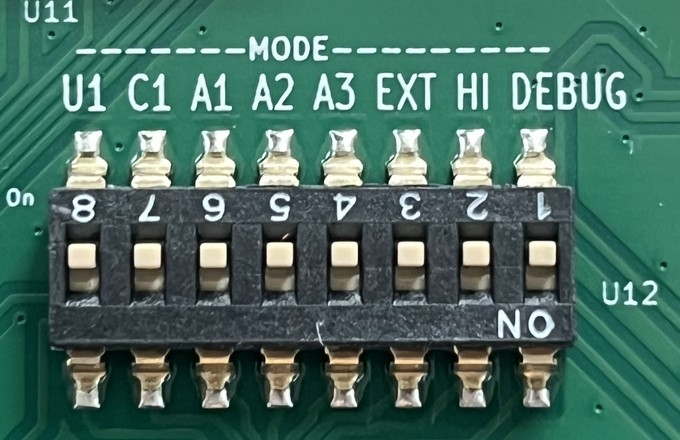
\includegraphics[width=\linewidth]{rangee_mode.jpg}\par
{\footnotesize Figure 2 : rangée MODE, tous les switches sur OFF}
\end{minipage}\hfill
\begin{minipage}[t]{0.63\textwidth}
\vspace{0pt}\small
\begin{tabularx}{\linewidth}{@{}>{\bfseries}p{1.9cm}L>{\raggedright\arraybackslash}p{2.6cm}@{}}
\toprule
\normalfont Switch & Fonction & Position conseillée \\
\midrule
U1 & Mode manuel : planning réglé par les switches d'heures et de jours (voir section 5). & OFF \\
C1 & Test des lumières, avec \sw{DEBUG} sur ON : les voies d'éclairage et le flash s'allument en boucle, à tour de rôle. Arrêt par redémarrage. & OFF \\
A1, A2, A3 & Réservés (sélection des voies d'attraction). Sans effet avec le logiciel 5.2.1. & OFF \\
EXT & Réservé (sortie d'attraction externe). Sans effet avec le logiciel 5.2.1. & OFF \\
HI & Réservé (alimentation secteur). Sans effet avec le logiciel 5.2.1. & OFF \\
DEBUG & Mode réglage : réseau wifi et page de réglage. & ON pour régler, OFF en service \\
\bottomrule
\end{tabularx}
\end{minipage}

% ---------------------------------------------------------------- Page 4
\newpage
\section{Paramétrage avec un téléphone}
\begin{minipage}[t]{0.37\textwidth}
\vspace{0pt}
\subsection{Connexion}
\begin{enumerate}
  \item Placer \sw{Active} et \sw{DEBUG} sur ON.
  \item Brancher la batterie.
  \item Attendre 2 à 3 minutes.
  \item Dans les réglages wifi du téléphone, sélectionner le réseau \texttt{Mothbox-}\textit{nom}.\\Mot de passe : \texttt{lunaluna}.
  \item La page de réglage s'ouvre automatiquement. À défaut, saisir \texttt{192.168.50.5} dans le navigateur.
\end{enumerate}
\remarque{Le téléphone peut signaler l'absence d'accès à Internet. Choisir de rester connecté à ce réseau.}
La langue de la page suit celle du téléphone. Le bouton FR/EN, en haut à droite, permet de la changer.

La page comporte quatre étapes, accessibles par les onglets 1 à 4 ou par le bouton \emph{Étape suivante}.
\end{minipage}\hfill
\begin{minipage}[t]{0.28\textwidth}
\vspace{0pt}\centering
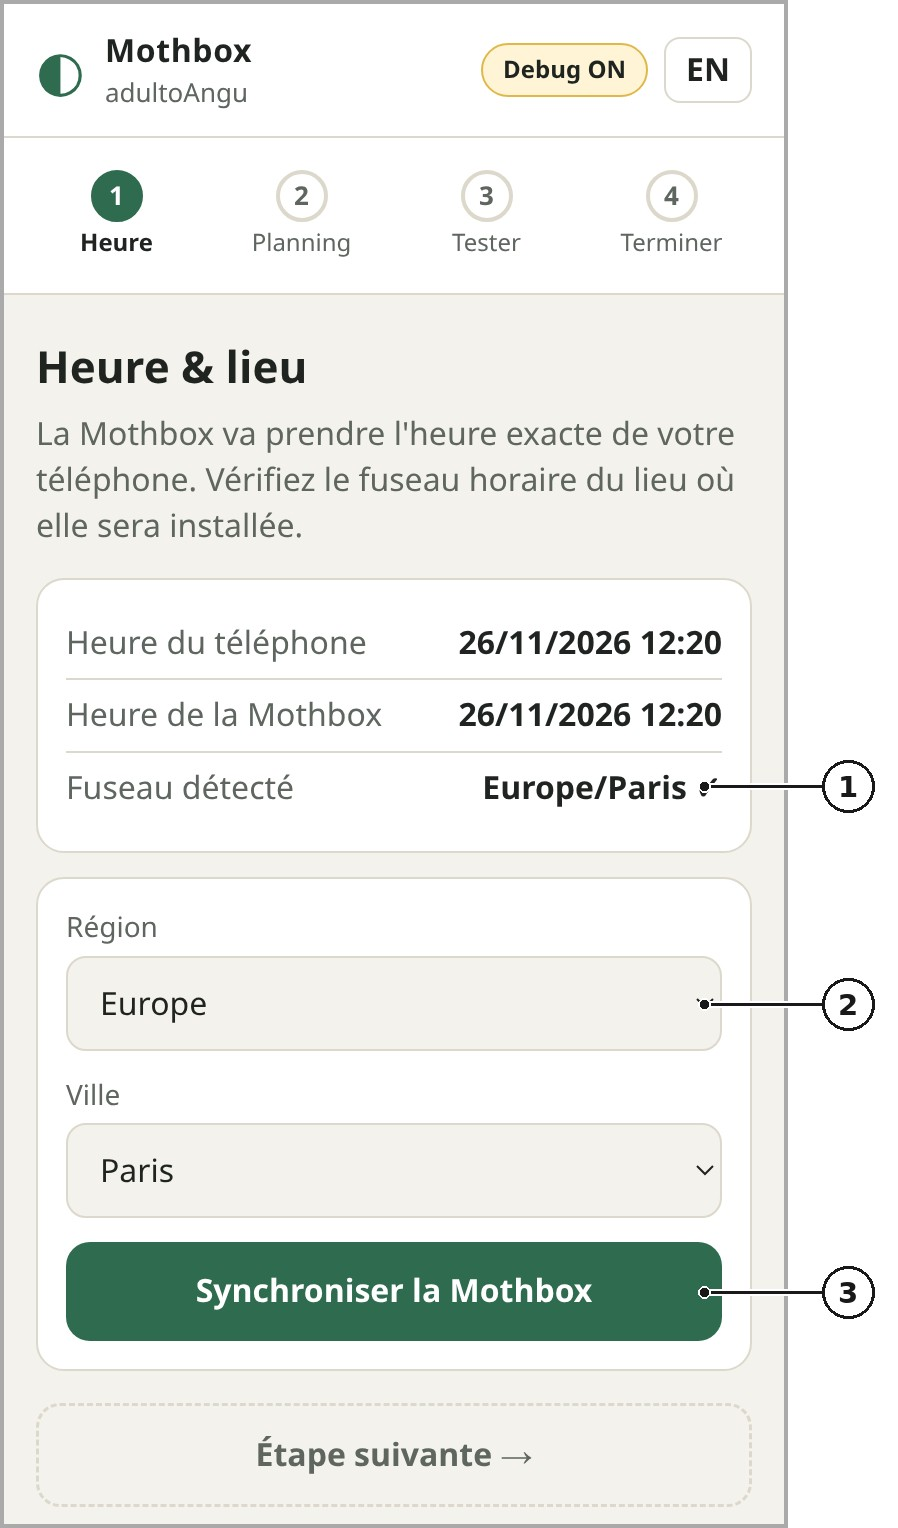
\includegraphics[width=\linewidth]{ecran1.jpg}\par
{\footnotesize Figure 3 : étape 1, heure et lieu}
\end{minipage}\hfill
\begin{minipage}[t]{0.29\textwidth}
\vspace{0pt}
\subsection{Étape 1 : heure et lieu}
La Mothbox reprend l'heure du téléphone.
\begin{enumerate}
  \item Vérifier le fuseau horaire détecté \rep{1}.
  \item Si le lieu d'installation est dans un autre fuseau, choisir la région et la ville \rep{2}.
  \item Appuyer sur \emph{Synchroniser la Mothbox} \rep{3}. L'écart corrigé s'affiche.
\end{enumerate}
\remarque{Si aucun fuseau n'est détecté, le bouton reste inactif tant qu'aucune ville n'est choisie.}
\end{minipage}

% ---------------------------------------------------------------- Page 5
\newpage
\begin{minipage}[t]{0.25\textwidth}
\vspace{0pt}\centering
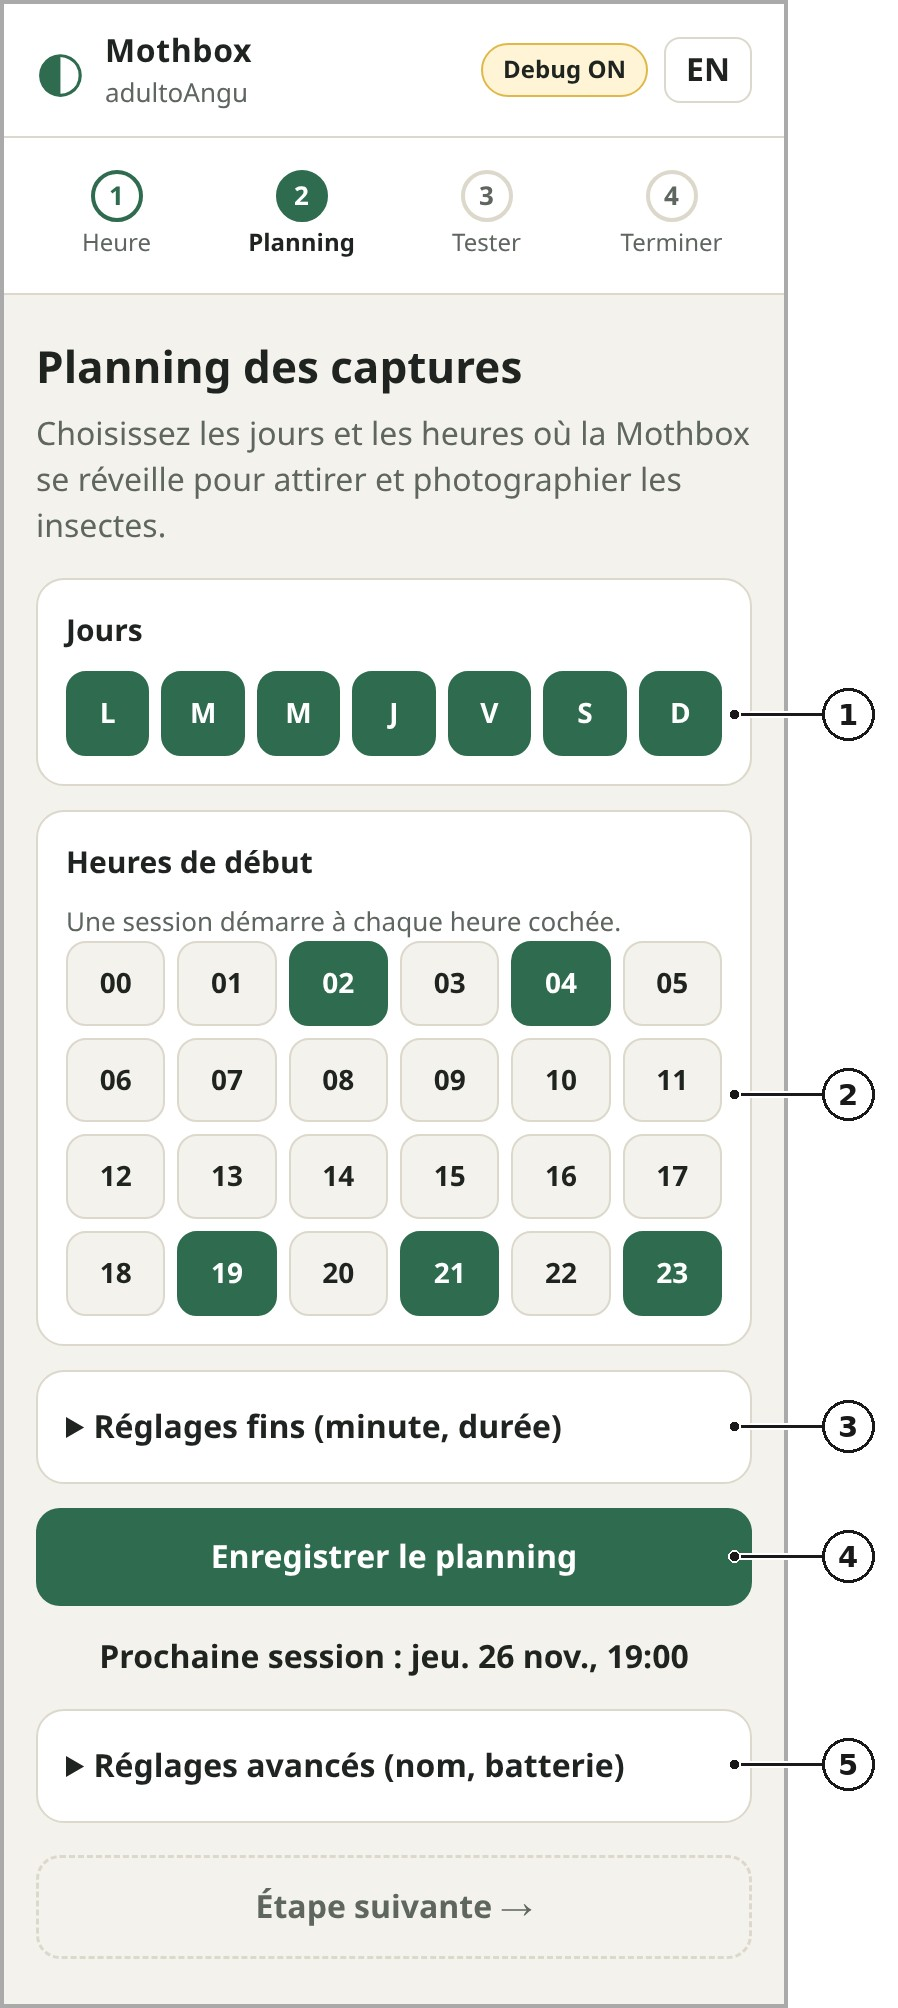
\includegraphics[width=\linewidth]{ecran2.jpg}\par
{\footnotesize Figure 4 : étape 2, planning}
\end{minipage}\hfill
\begin{minipage}[t]{0.23\textwidth}
\vspace{0pt}
\subsection*{Étape 2 : planning}
\begin{enumerate}
  \item Sélectionner les jours de capture \rep{1}.
  \item Sélectionner les heures de début \rep{2}. Une session démarre à chaque heure sélectionnée.
  \item Si nécessaire, régler la minute de départ et la durée d'une session \rep{3} (59 min par défaut).
  \item Appuyer sur \emph{Enregistrer le planning} \rep{4}. La prochaine session s'affiche.
\end{enumerate}
Les \emph{Réglages avancés} \rep{5} permettent de modifier le nom de la Mothbox et les caractéristiques de la batterie.
\end{minipage}\hfill
\begin{minipage}[t]{0.25\textwidth}
\vspace{0pt}\centering
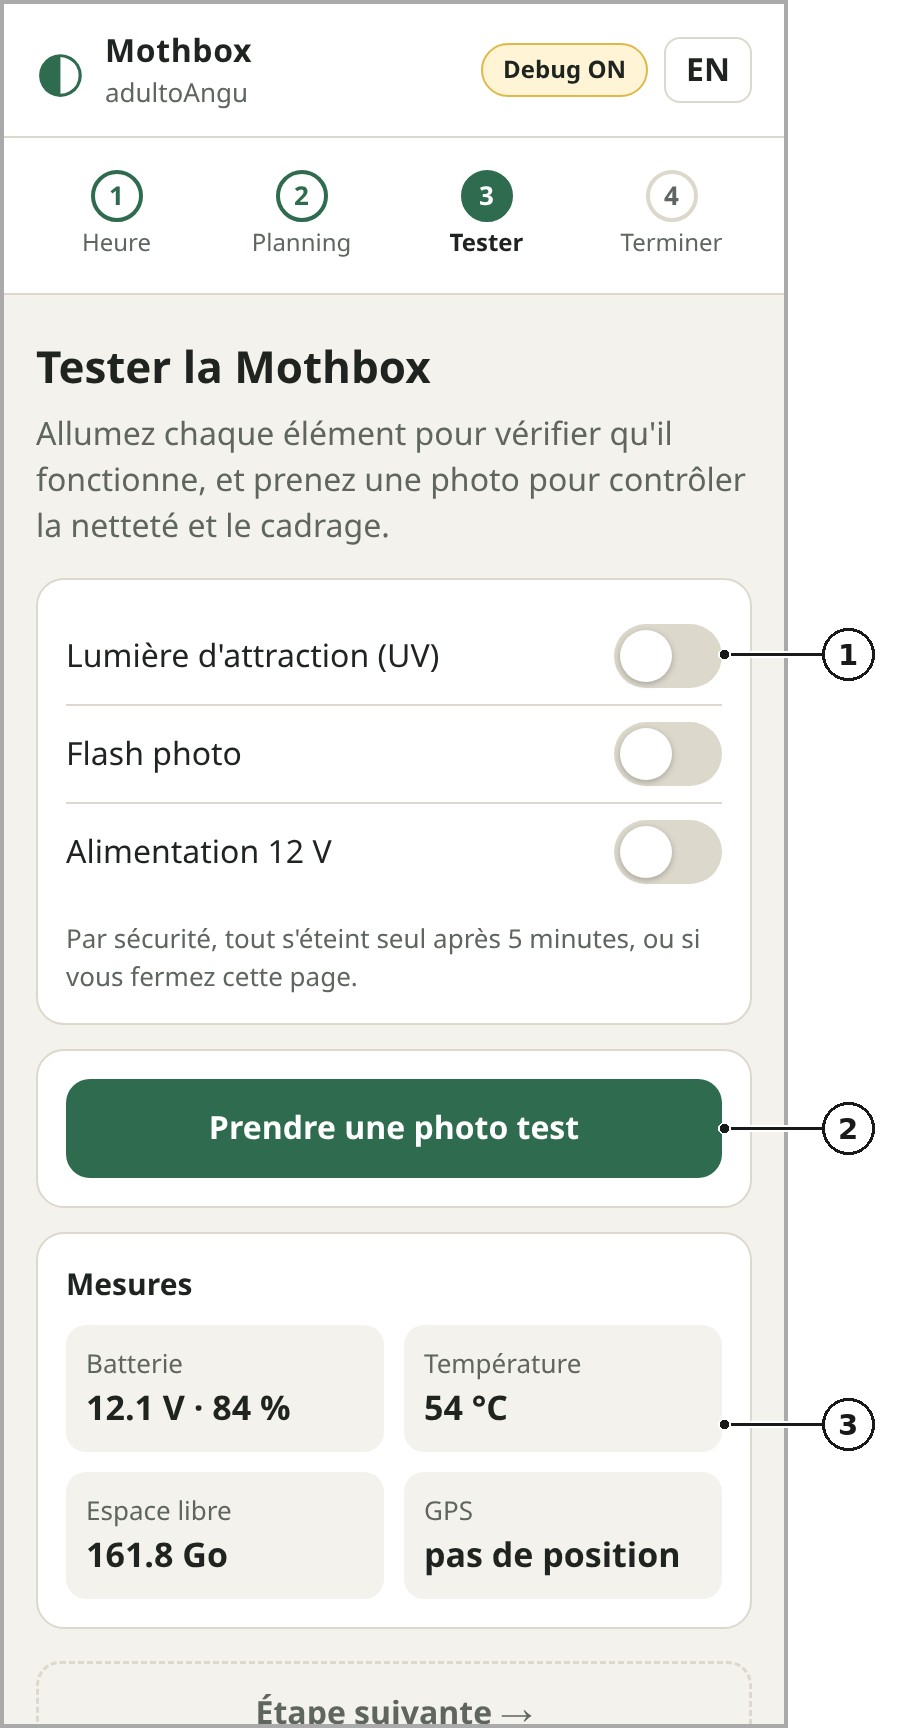
\includegraphics[width=\linewidth]{ecran3.jpg}\par
{\footnotesize Figure 5 : étape 3, tests}
\end{minipage}\hfill
\begin{minipage}[t]{0.23\textwidth}
\vspace{0pt}
\subsection*{Étape 3 : tests}
\begin{enumerate}
  \item Allumer puis éteindre la lumière d'attraction, le flash et l'alimentation 12\,V \rep{1}.
  \item Appuyer sur \emph{Prendre une photo test} \rep{2}. Vérifier que le drap est net et occupe toute l'image.
  \item Contrôler les mesures \rep{3} : batterie, température, espace libre, position GPS.
\end{enumerate}
\remarque{Les sorties s'éteignent automatiquement après 5 minutes, ou 30 secondes après la fermeture de la page.}
\end{minipage}

% ---------------------------------------------------------------- Page 6
\newpage
\begin{minipage}[t]{0.22\textwidth}
\vspace{0pt}\centering
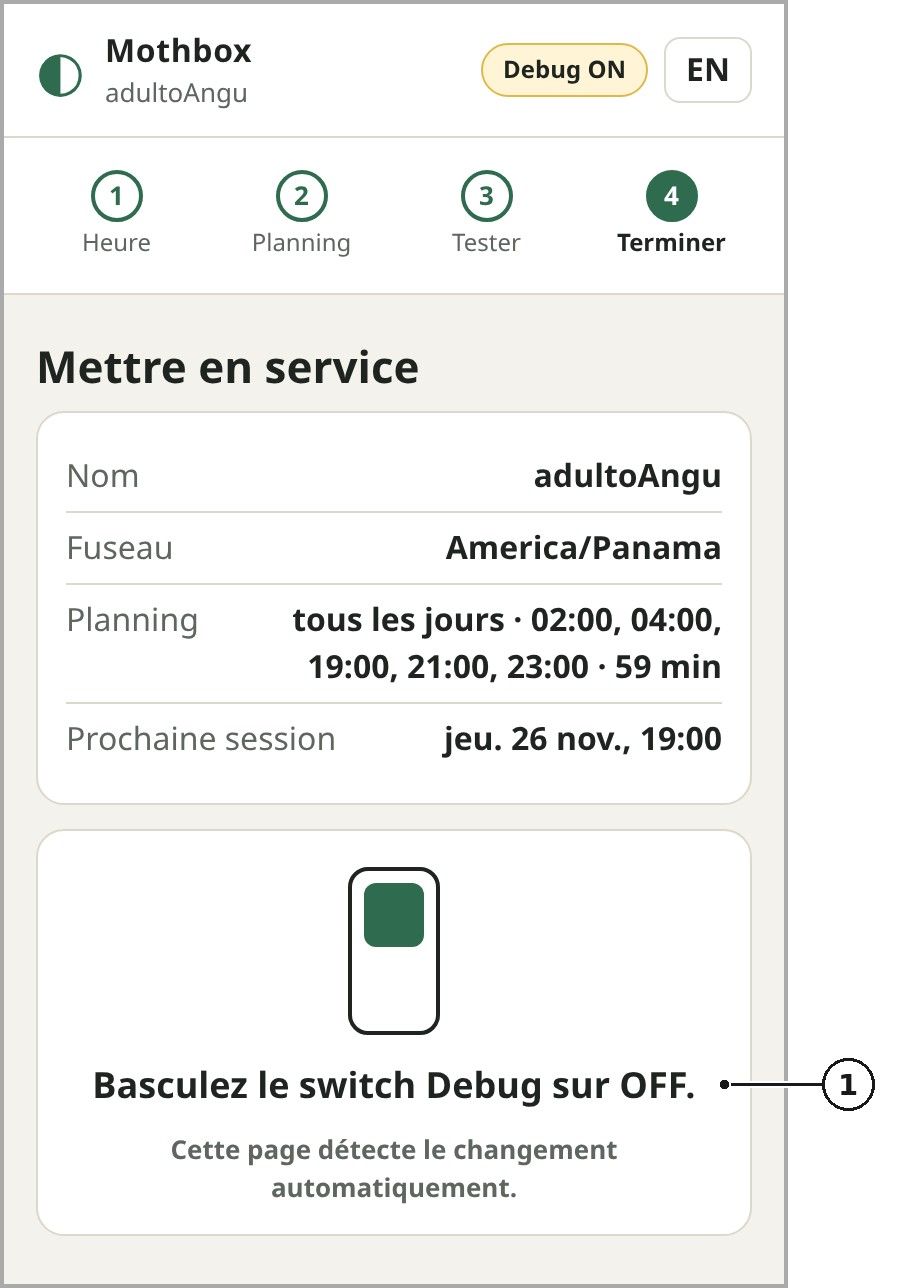
\includegraphics[width=\linewidth]{ecran4.jpg}\par\vspace{4pt}
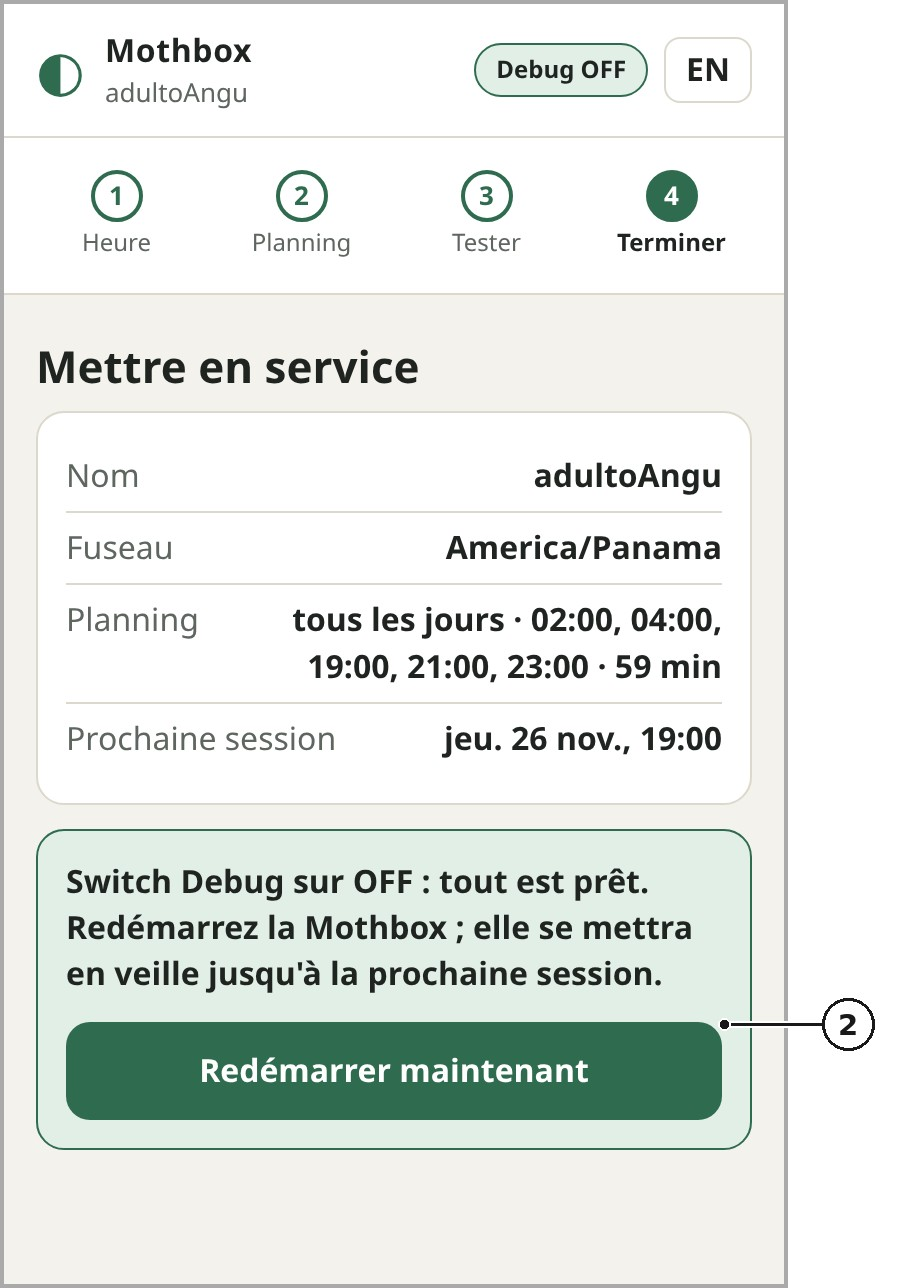
\includegraphics[width=\linewidth]{ecran4_pret.jpg}\par
{\footnotesize Figure 6 : étape 4, mise en service}
\end{minipage}\hfill
\begin{minipage}[t]{0.33\textwidth}
\vspace{0pt}
\subsection*{Étape 4 : mise en service}
La page récapitule le nom, le fuseau, le planning et la prochaine session.
\begin{enumerate}
  \item Placer \sw{DEBUG} sur OFF \rep{1}, sans débrancher la batterie. Laisser \sw{Active} sur ON.
  \item Attendre que la page détecte le changement, puis appuyer sur \emph{Redémarrer maintenant} \rep{2}.
\end{enumerate}
La Mothbox redémarre, coupe son réseau wifi et se met en veille jusqu'à la prochaine session. La page peut être fermée.
\avert{Attention}{Si la page indique que le switch Active est sur OFF, le replacer sur ON. Dans cette position, la Mothbox s'éteindrait à chaque réveil sans effectuer de capture.}
\end{minipage}\hfill
\begin{minipage}[t]{0.40\textwidth}
\vspace{0pt}
\section{Mode manuel}
Le planning peut être réglé directement sur la carte, sans téléphone.
\begin{enumerate}
  \item Placer \sw{U1} sur ON.
  \item Placer sur ON les switches des heures de début et des jours souhaités.
  \item Placer \sw{Active} sur ON et \sw{DEBUG} sur OFF.
  \item Redémarrer la Mothbox.
\end{enumerate}
En mode manuel, chaque session démarre à l'heure pile et dure 59 minutes. Sans heure sélectionnée, la Mothbox applique 19\,h, 21\,h, 23\,h, 2\,h et 4\,h ; sans jour sélectionné, elle fonctionne tous les jours.

\begin{minipage}[t]{0.42\linewidth}
\vspace{0pt}
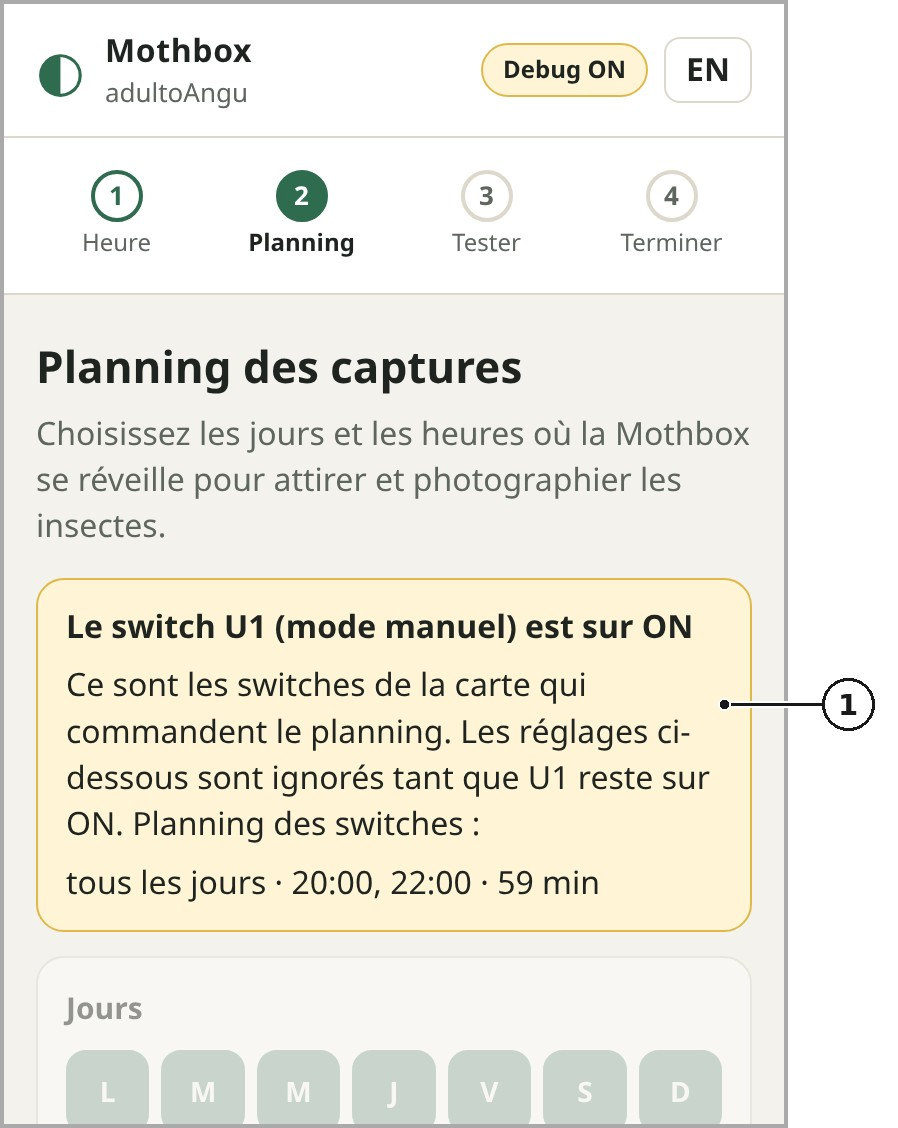
\includegraphics[width=\linewidth]{ecran2_u1.jpg}
\end{minipage}\hfill
\begin{minipage}[t]{0.54\linewidth}
\vspace{0pt}\small
Tant que \sw{U1} est sur ON, la page de réglage affiche un bandeau \rep{1} et le planning lu sur les switches. Ses propres réglages de planning sont alors ignorés.
\end{minipage}
\end{minipage}

% ---------------------------------------------------------------- Page 7
\newpage
\section{Dépannage}
\small
\begin{tabularx}{\linewidth}{@{}>{\raggedright\arraybackslash}p{5.2cm}>{\raggedright\arraybackslash}p{6.6cm}L@{}}
\toprule
\normalsize\bfseries Problème & \normalsize\bfseries Cause possible & \normalsize\bfseries Solution \\
\midrule
Aucun réseau \texttt{Mothbox-}\textit{nom} & Démarrage en cours. & Attendre 3 minutes. \\
 & \sw{Active} ou \sw{DEBUG} sur OFF. & Placer les deux sur ON, puis redémarrer. \\
 & Nom de réseau par défaut. & Rechercher le réseau \texttt{mothboxwifi}. \\
\midrule
Connecté, mais la page ne s'ouvre pas & Ouverture automatique bloquée par le téléphone. & Saisir \texttt{192.168.50.5} dans le navigateur. \\
\midrule
Le téléphone se déconnecte & Le téléphone recherche un réseau avec Internet. & Choisir de rester connecté ; désactiver temporairement les données mobiles. \\
\midrule
Message \og La carte n'a pas répondu \fg{} & Lumière ou flash mal branché. & Vérifier les câbles sur les borniers, puis réessayer. \\
\midrule
Message \og La caméra n'a pas répondu \fg{} & Nappe de la caméra mal insérée. & Vérifier la nappe aux deux extrémités, puis réessayer. \\
\midrule
La page attend le passage de DEBUG sur OFF & Mauvais switch basculé. & Basculer le dernier switch de la rangée MODE, marqué DEBUG. \\
\midrule
Captures aux mauvaises heures & Fuseau horaire incorrect. & Refaire l'étape 1. \\
 & \sw{U1} sur ON. & Placer \sw{U1} sur OFF si le planning a été réglé sur la page. \\
\midrule
Aucune capture & \sw{Active} sur OFF ou \sw{DEBUG} sur ON. & Placer \sw{Active} sur ON et \sw{DEBUG} sur OFF, puis redémarrer. \\
\bottomrule
\end{tabularx}

% ---------------------------------------------------------------- Page 8
\newpage
\begin{minipage}[t]{0.52\textwidth}
\vspace{0pt}
\section{Préparation d'une carte SD}
La préparation se fait avec le logiciel gratuit Raspberry Pi Imager (Windows, macOS, Linux), disponible sur \texttt{raspberrypi.com/software}.

Fichier à utiliser : \texttt{mothbox\_Pro\_Pi5\_v5.2.1-webui\_2026-11-27-v4.img.xz}, à télécharger sur \texttt{github.com/Tom-PSLD/mothbox-webui/releases}. Ne pas le décompresser.
\begin{enumerate}
  \item Insérer une carte SD de 16\,Go minimum dans l'ordinateur.
  \item Dans Raspberry Pi Imager, choisir l'appareil \emph{Raspberry Pi 5}.
  \item Dans \emph{Système d'exploitation}, choisir \emph{Utiliser une image personnalisée} (en bas de la liste), puis sélectionner le fichier.
  \item Dans \emph{Stockage}, sélectionner la carte SD.
  \item À la question sur la personnalisation de l'OS, répondre \emph{Non}.
  \item Attendre la fin de l'écriture et de la vérification (environ 10 minutes), puis retirer la carte.
\end{enumerate}
\avert{Attention}{Toutes les données de la carte SD sont effacées. Vérifier la taille du support sélectionné avant de lancer l'écriture.}
\avert{Attention}{Ne pas personnaliser l'OS (utilisateur, mot de passe, wifi) : la Mothbox pourrait ne plus créer son propre réseau.}
\end{minipage}\hfill
\begin{minipage}[t]{0.43\textwidth}
\vspace{0pt}
\section{Caractéristiques}
\small
\begin{tabularx}{\linewidth}{@{}>{\raggedright\arraybackslash}p{4.2cm}L@{}}
\toprule
Logiciel & 5.2.1-webui, basé sur Mothbox 5.2.1 \\
Matériel compatible & Mothbox Pro, carte v5.0.x, Raspberry Pi 5 \\
\midrule
Réseau wifi (mode réglage) & \texttt{Mothbox-}\textit{nom} \\
Mot de passe & \texttt{lunaluna} \\
Adresse de la page & \texttt{192.168.50.5} \\
Langues & français, anglais \\
\midrule
Jours programmables & lundi à dimanche \\
Heures de début & 00\,h à 23\,h, plusieurs par jour \\
Durée d'une session & 1 à 1439 minutes (59 par défaut) \\
Planning en mode manuel & heure pile, 59 minutes \\
\midrule
Extinction automatique des sorties & 5 minutes après allumage \\
 & 30 secondes après fermeture de la page \\
Horloge & conservée hors tension (pile RTC) \\
\bottomrule
\end{tabularx}
\end{minipage}

\end{document}
